%%===========================================================%%
%%                                                           %%
%%                     DE/DX CORRECTION                      %%
%%                                                           %%
%%===========================================================%%


\chapter{\texorpdfstring{d$\bm{E}$/d$\bm{x}$}{dE/dx} correction}\label{chap:dEdxCorrection}

Particle identification in our analyses is done using merged information from the TPC (specific energy loss of tracks $dE/dx$) and from the TOF (time of hit macthed to TPC track). As can be seen in Fig.~\ref{fig:dEdxDataVsMC}, $dE/dx$ information from the MC events simulated in STARsim (in red) poorely matches the data points (black). This results e.g. in large systematic error of estimate of particle identification efficiency.

This problem was discussed under ticket \#3272~(Ref.~\cite{dedxTicket}). There were trials to improve the TPC calibration in simulation, but the problem remained. It was finally concluded that the origin of the problem lies in the model of energy loss used in the STARsim, therefore any further action was postponed. 

In order to tune simulated reposponse of the TPC in terms of $dE/dx$, hence also reduce the systematic uncertainty related to particle identification, a correction method was developed based on proper transformation (recalculation) of simulated $dE/dx$ to obtain new $dE/dx$ whose distribution matches the data.

It is possible to transform dE/dx in MC to make it follow the shape of dE/dx in the data. 
We know that $n^{\sigma}_{X}$ (where $X=\pi, K, p$, ...) variable follows a gaussian distribution (for particle X)
 \[n^{\sigma}_{X} = \Big( \ln{\frac{dE/dx}{\langle dE/dx\rangle_{X}}} \Big) / \sigma_{dE/dx},~~~~~f(n^{\sigma}_{X}) = \mathcal{N}(n^{\sigma}_{X}; \mu=0,\sigma=1)\]
therefore $dE/dx$ itself follows log-normal distribution:
\[f(dE/dx) = \mathcal{L}og\mathcal{N}(dE/dx; \mu=\langle dE/dx\rangle,\sigma=\sigma_{dE/dx}) = \frac{1}{\sqrt{2\pi}\cdot \sigma\cdot dE/dx}e^{-\frac{\ln^{2}{\frac{dE/dx}{\langle dE/dx\rangle}}}{2\sigma^{2}}}\]
The transformation we want to apply should preserve the shape of $dE/dx$ (so that it is still described by $\mathcal{L}og\mathcal{N}$), however it should change $\mu$ and $\sigma$ so that these values are euqal to those seen in the data. The transformation that satisfies above postulate is
\[dE/dx' = c\cdot (dE/dx)^{a}\]
Parameters of the distribution $\mathcal{L}og\mathcal{N}(dE/dx')$ would be then
\[\mu' = c\cdot\mu^{a},~~~~\sigma' = a\cdot\sigma\]
From above we get formulae for parameters of the transformation:
\[a=\sigma'/\sigma,~~~~c = \frac{\mu'}{\mu^{a}}\]

AlternativeToCrystallBall~\cite{AlternativeToCrystallBall}~Eq.~\eqref{eq:expTail}

\begin{equation}\label{eq:expTail}
	f(dE/dx)=\left\{
                \begin{array}{ll}
                  \frac{A}{\sqrt{2\pi}\cdot \sigma\cdot dE/dx}\exp{\Bigg(-\frac{1}{2}\Big(\frac{\ln{\frac{dE/dx}{\langle dE/dx\rangle}}}{\sigma}\Big)^{2}\Bigg)} & \textrm{for}~\frac{\ln{\frac{dE/dx}{\langle dE/dx\rangle}}}{\sigma} \leq k \\
                  \frac{A}{\sqrt{2\pi}\cdot \sigma\cdot dE/dx}\exp{\Bigg(-k\cdot \frac{\ln{\frac{dE/dx}{\langle dE/dx\rangle}}}{\sigma} + \frac{1}{2}k^{2} - k^{-1}\left(\frac{\frac{\ln{\frac{dE/dx}{\langle dE/dx\rangle}}}{\sigma}}{k}-1\right)^{k} \Bigg)} & \textrm{for}~\frac{\ln{\frac{dE/dx}{\langle dE/dx\rangle}}}{\sigma} > k
                \end{array}
              \right.
\end{equation}



%---------------------------
\begin{figure}[hb]
\centering
\parbox{0.495\textwidth}{
  \centering
  \includegraphics[width=\linewidth,page=4]{graphics/dedx/dEdx_fitPerMomentumBin_3rdIteration.pdf}\\
  \includegraphics[width=\linewidth,page=14]{graphics/dedx/dEdx_fitPerMomentumBin_3rdIteration.pdf}\\
  \includegraphics[width=\linewidth,page=24]{graphics/dedx/dEdx_fitPerMomentumBin_3rdIteration.pdf}\\
  \includegraphics[width=\linewidth,page=34]{graphics/dedx/dEdx_fitPerMomentumBin_3rdIteration.pdf}
}~
\parbox{0.495\textwidth}{
  \centering
  \includegraphics[width=\linewidth,page=9]{graphics/dedx/dEdx_fitPerMomentumBin_3rdIteration.pdf}\\
  \includegraphics[width=\linewidth,page=19]{graphics/dedx/dEdx_fitPerMomentumBin_3rdIteration.pdf}\\
  \includegraphics[width=\linewidth,page=29]{graphics/dedx/dEdx_fitPerMomentumBin_3rdIteration.pdf}\\
  \includegraphics[width=\linewidth,page=39]{graphics/dedx/dEdx_fitPerMomentumBin_3rdIteration.pdf}
}%
\caption[Fits to dE/dx spectra from the data.]{Fits of sum of functions from Eq.~\eqref{eq:expTail} corresponding to different particle species to dE/dx spectra from the data in a few momentum bins.}\label{fig:dEdxFits}
\end{figure}
%---------------------------



%---------------------------
\begin{figure}[hb]
\centering
\parbox{0.4725\textwidth}{
  \centering
  \begin{subfigure}[b]{\linewidth}{
                \subcaptionbox{\label{fig:dEdxMeanOffsetMC}}{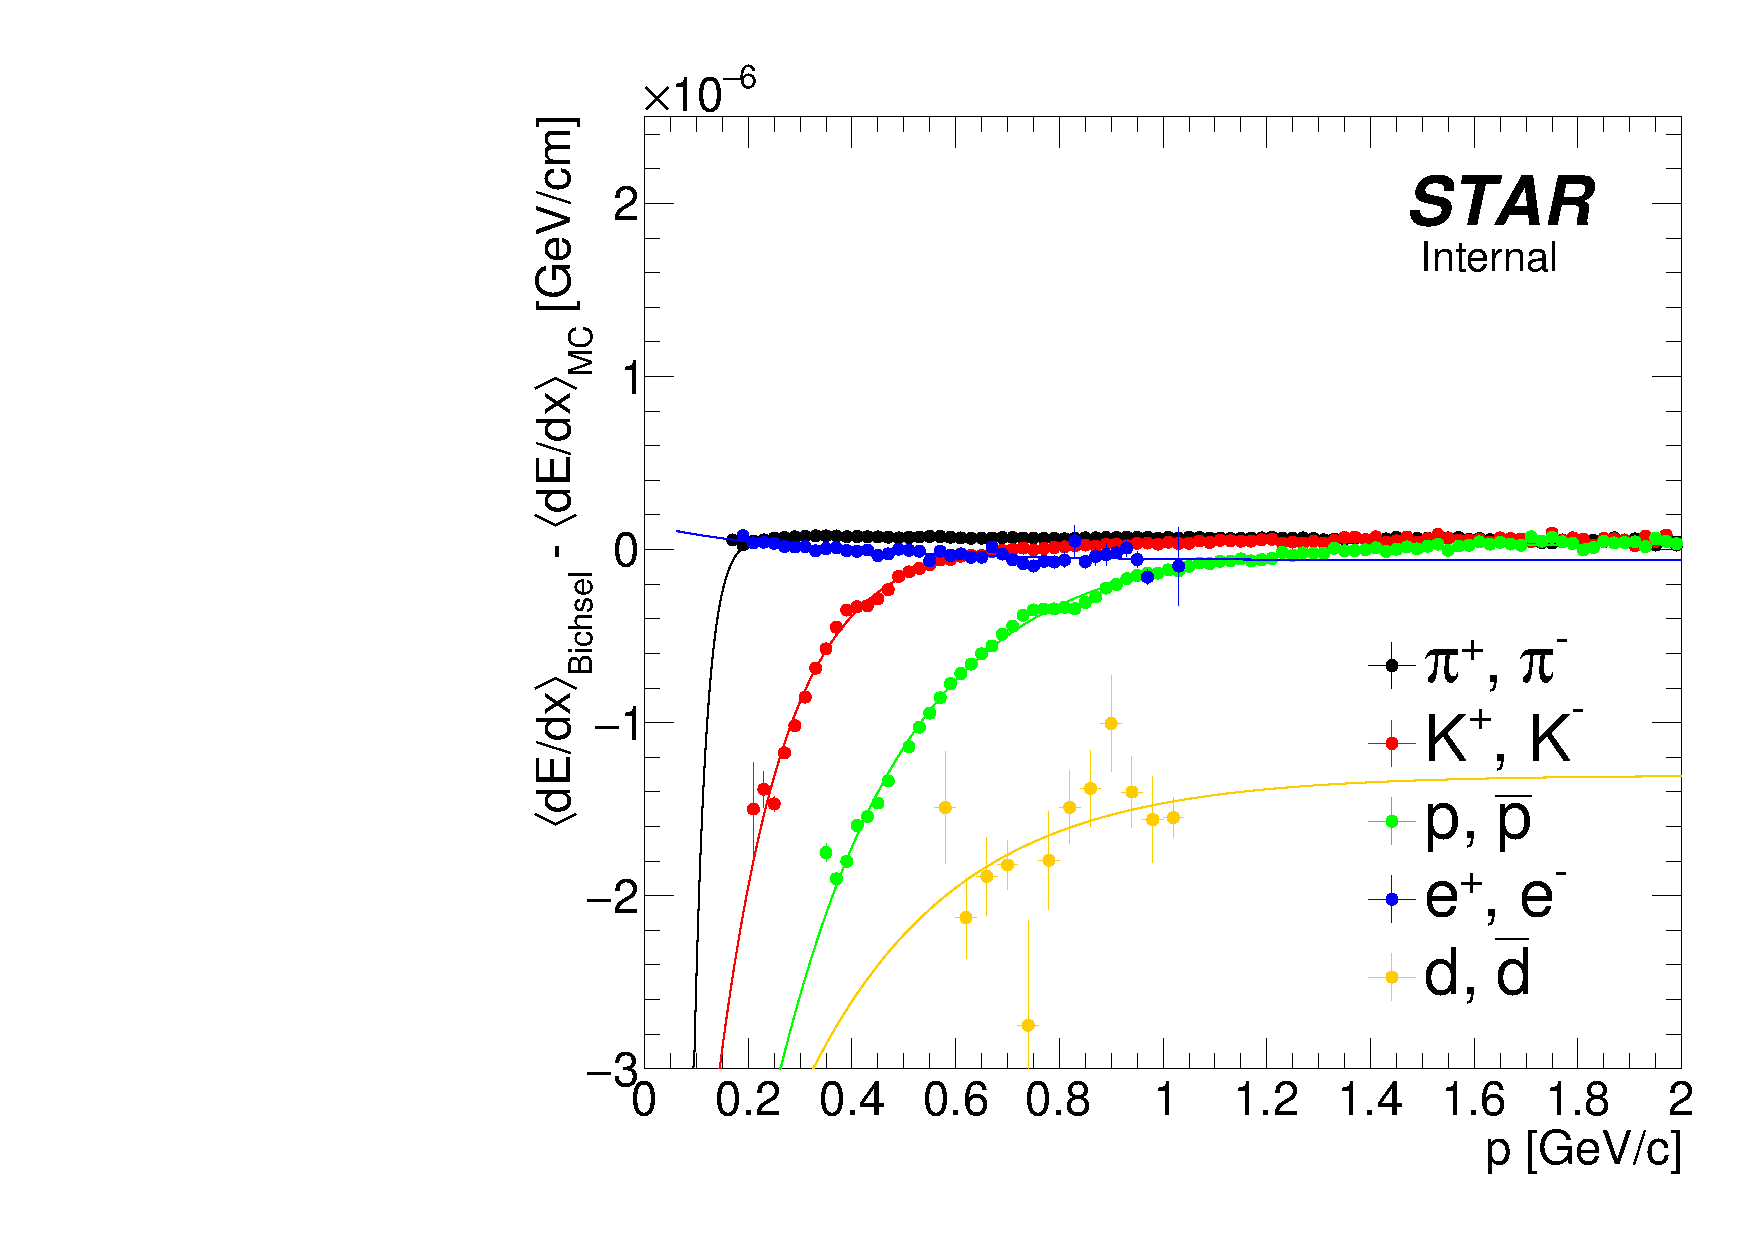
\includegraphics[width=\linewidth]{graphics/dedx/dEdxMeanOffset_allPIDs.pdf}\vspace*{-10pt}}}
  \end{subfigure}\\
  \begin{subfigure}[b]{\linewidth}\addtocounter{subfigure}{1}{
                \subcaptionbox{\label{fig:dEdxMeanOffsetData}}{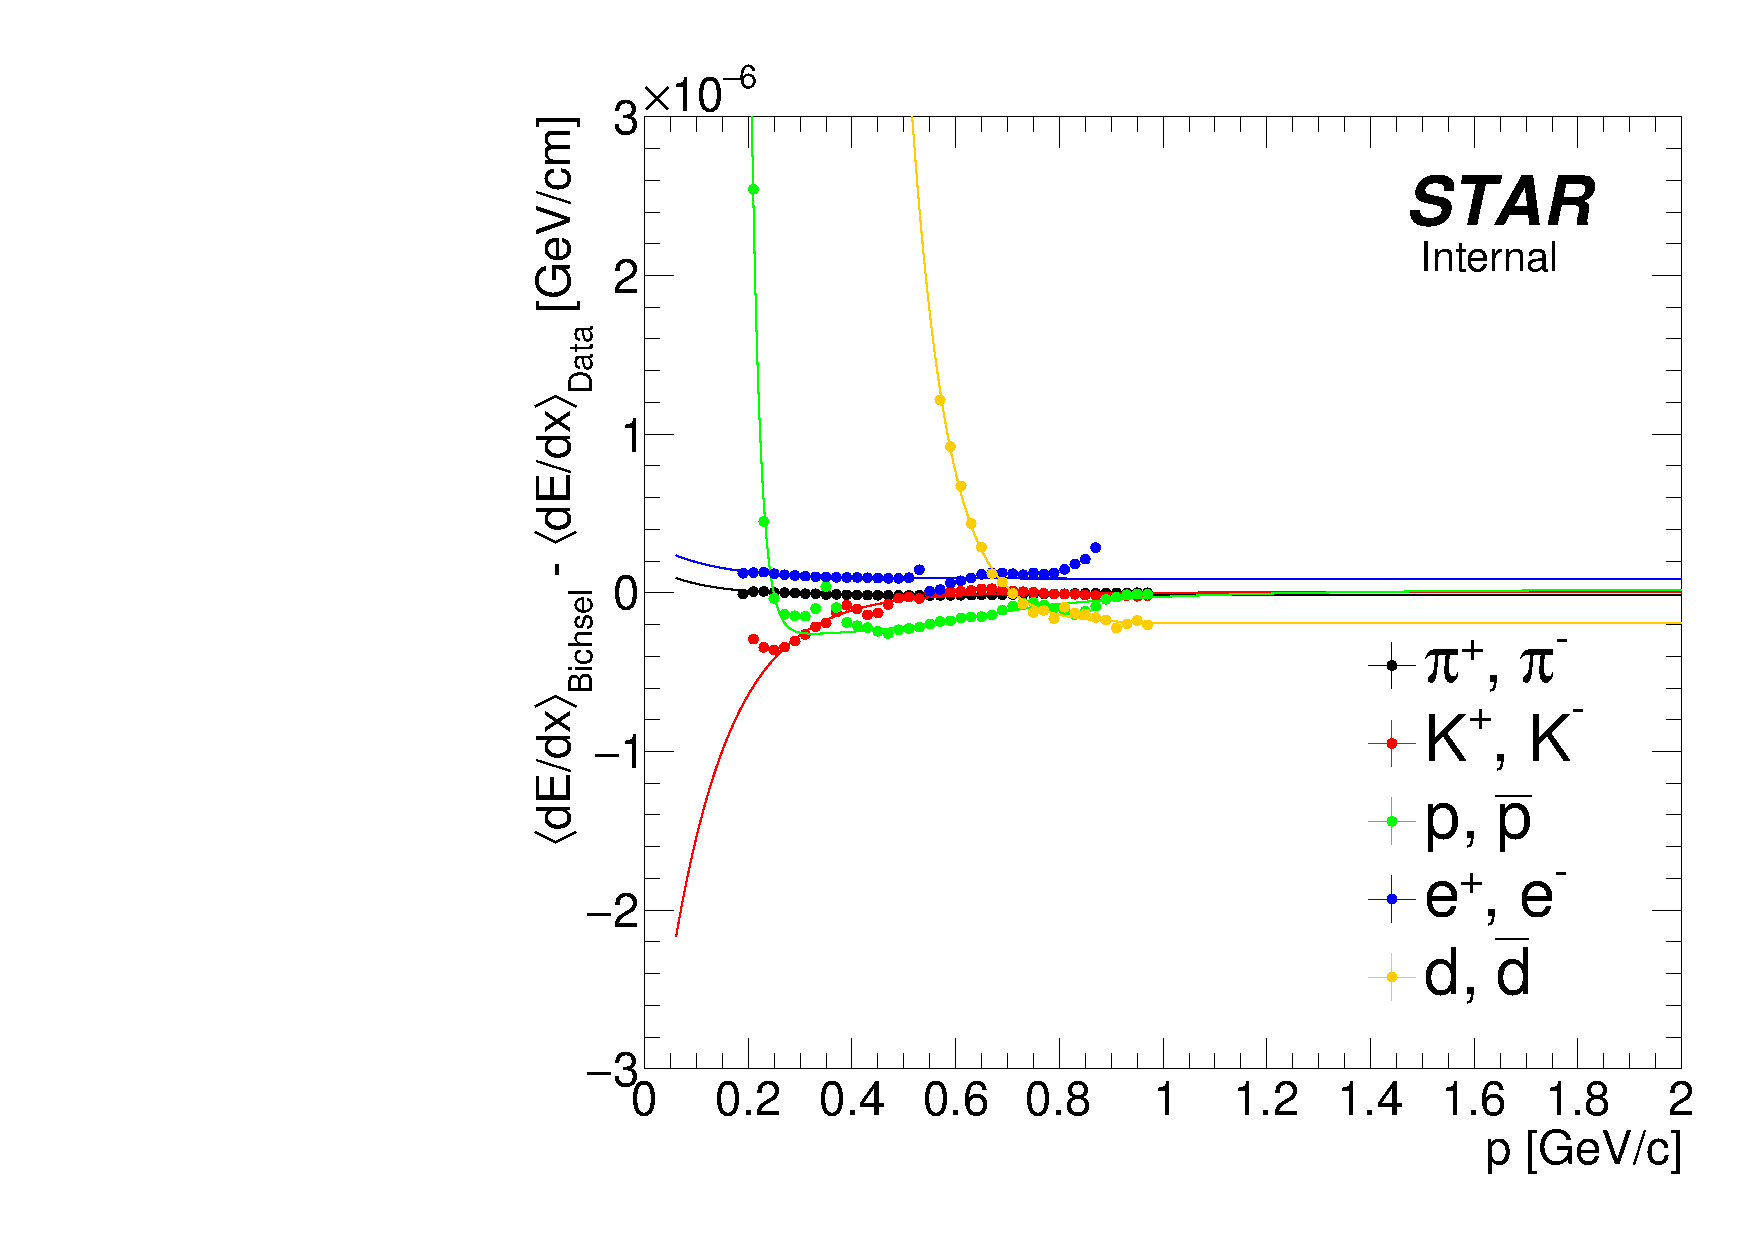
\includegraphics[width=\linewidth]{graphics/dedx/dEdxMeanOffset_allPIDs_data.pdf}\vspace*{-10pt}}}
  \end{subfigure}
}
\quad
\parbox{0.4725\textwidth}{
  \centering
  \begin{subfigure}[b]{\linewidth}\addtocounter{subfigure}{-2}{
                \subcaptionbox{\label{fig:dEdxWidthMC}}{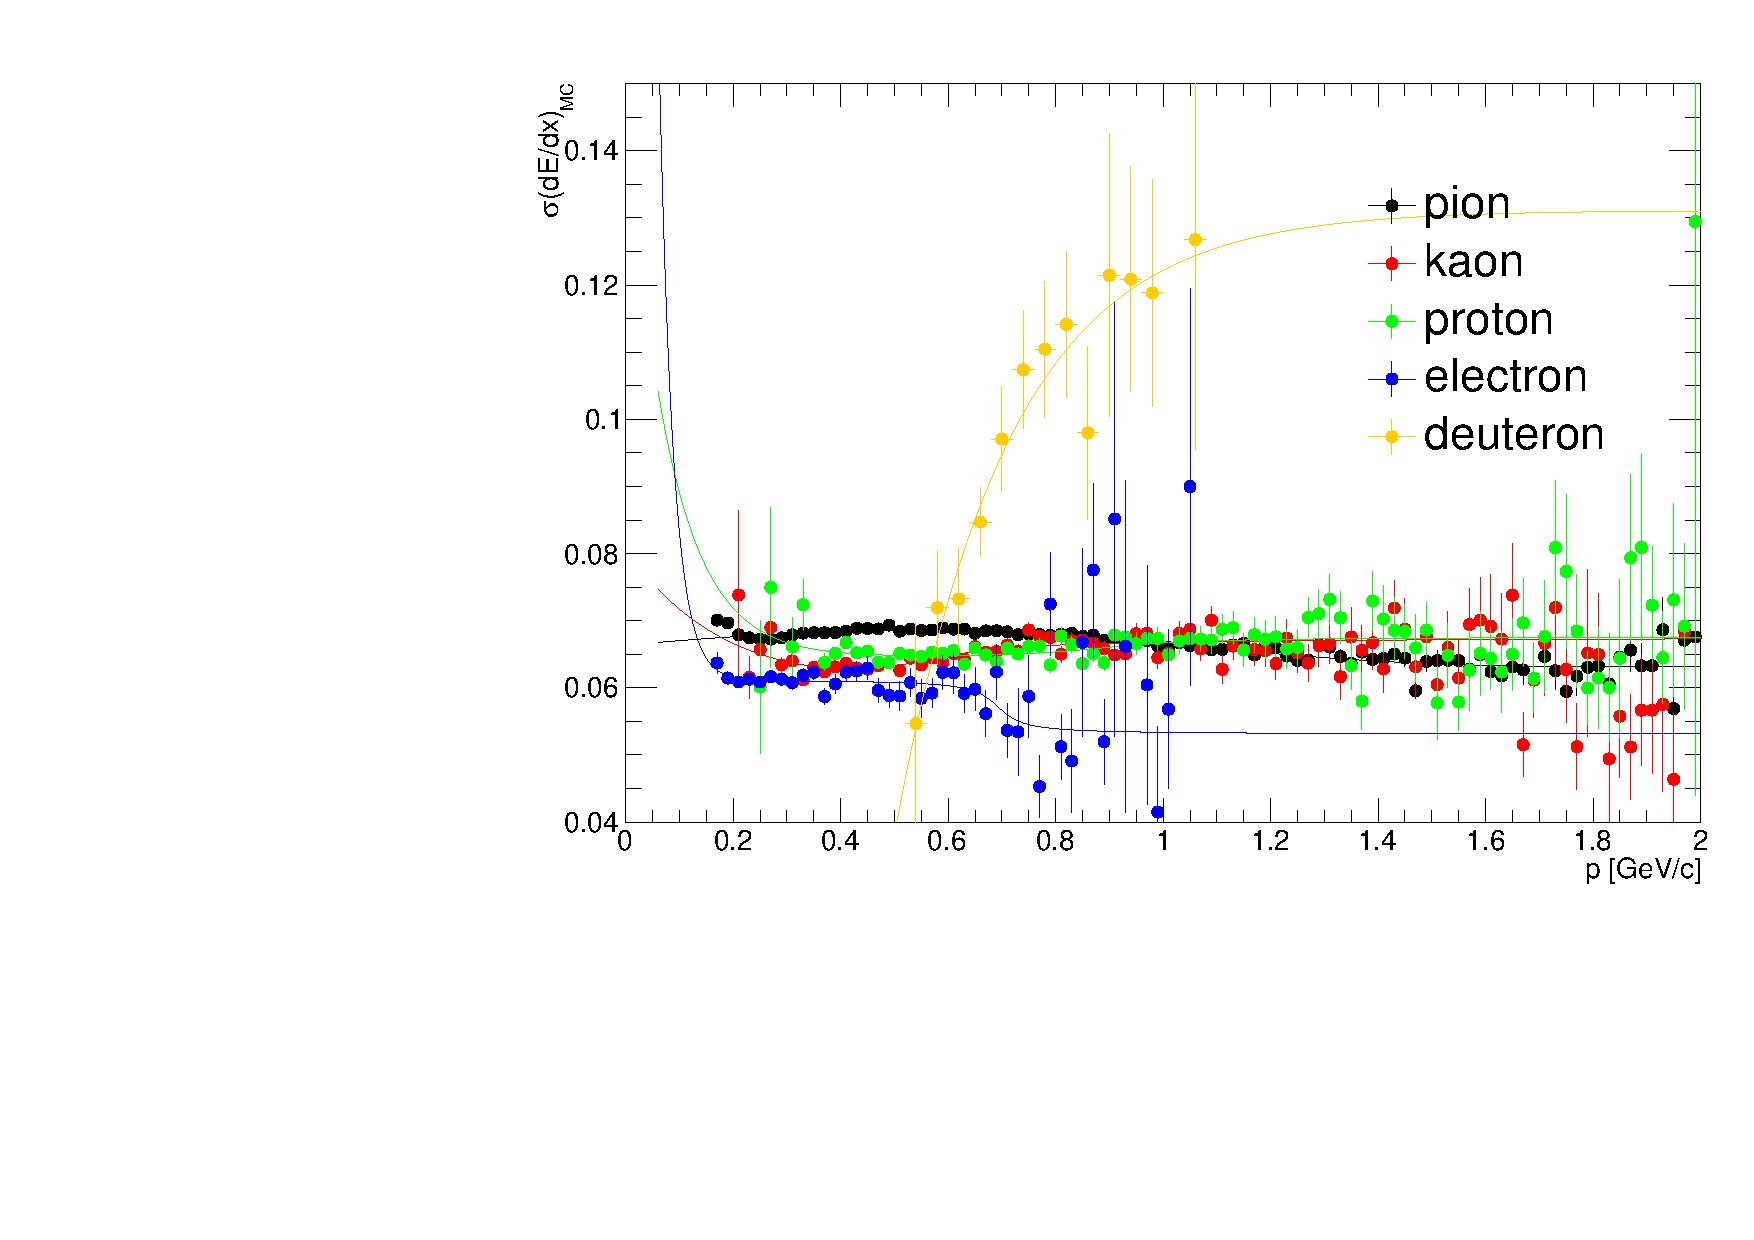
\includegraphics[width=\linewidth]{graphics/dedx/dEdxWidth_allPIDs.pdf}\vspace*{-10pt}}}
  \end{subfigure}\\
  \begin{subfigure}[b]{\linewidth}\addtocounter{subfigure}{1}{
                \subcaptionbox{\label{fig:dEdxWidthData}}{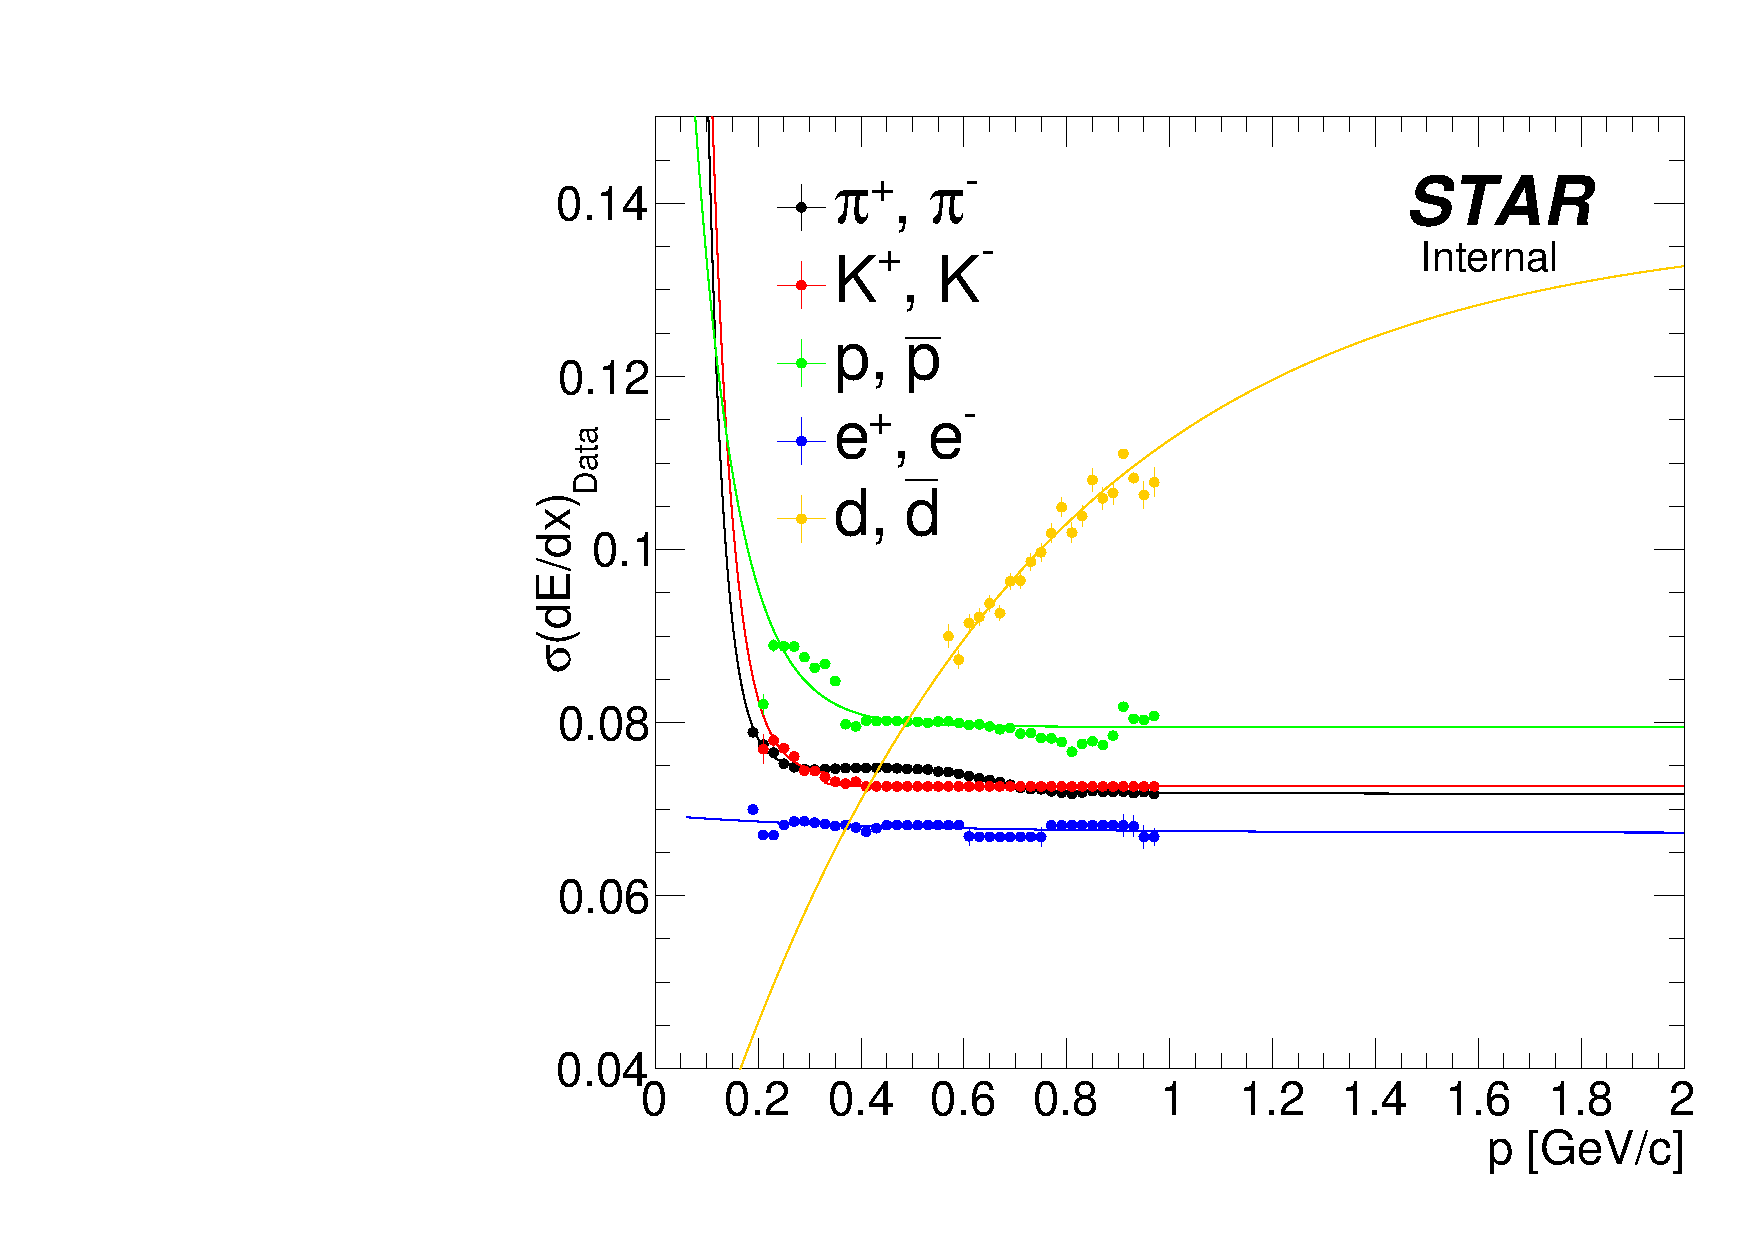
\includegraphics[width=\linewidth]{graphics/dedx/dEdxWidth_allPIDs_data.pdf}\vspace*{-10pt}}}
  \end{subfigure}
}%
\caption[Parameters of track dE/dx as a function of reconstructed momentum for a few particle species.]{Difference between MPV of dE/dx predicted by Bichsel parametrization and obtained from the fit of Eq.~\eqref{eq:expTail} to dE/dx distribution in the data (\ref{fig:dEdxMeanOffsetData}) and MC sample (\ref{fig:dEdxMeanOffsetMC}) and dE/dx width parameter in data (\ref{fig:dEdxWidthData}) and MC (\ref{fig:dEdxWidthMC}) as a function of reconstructed particle momentum for a few particle species. Solid lines represent fits to points of corresponding color.}\label{fig:dEdxParametersMC}
\end{figure}
%---------------------------


\begin{equation}\label{eq:dEdxParametrization}
	g(p) = P_{1} + P_{2}\cdot \exp{\left(-P_{3}\cdot p\right)} + P_{4}\cdot \arctan{\big(P_{5}\cdot(p-P_{6})\big)}
\end{equation}



\begin{table}[ht!]\centering%
\subcaptionbox{\label{tab:dEdxParametersMC}}{%
 \begin{tabular}{r||c|c|c|c|c|c||c|c|c|c|c|c}%\hline
 \multirow{2}{*}{\textbf{PID}} &  \multicolumn{6}{c||}{\bm{$\langle dE/dx\rangle_{\textrm{\textbf{Bichsel}}} - \langle dE/dx\rangle_{\textrm{\textbf{MC}}}$}} & \multicolumn{6}{c}{\bm{$\sigma(dE/dx)_{\textrm{\textbf{MC}}}$}} \\ \cline{2-13}
  & $P_{1}$ & $P_{2}$ & $P_{3}$ & $P_{4}$ & $P_{5}$ & $P_{6}$ & $P_{1}$ & $P_{2}$ & $P_{3}$ & $P_{4}$ & $P_{5}$ & $P_{6}$ \\ \Xhline{2\arrayrulewidth}
$\bm{\pi^{\pm}}$ &\scriptsize 3.618e-8 &\scriptsize 5.838e-9 &\scriptsize 5.481 &\scriptsize          &\scriptsize         &\scriptsize          &\scriptsize 0.0809 &\scriptsize -0.023 &\scriptsize 0.450 &\scriptsize -7.84e-3 &\scriptsize 1.8489 &\scriptsize 1.04 \\ \hline
$\bm{K^{\pm}}$ &\scriptsize -1.01e-10 &\scriptsize -9.983e-6 &\scriptsize 7.581 &\scriptsize          &\scriptsize         &\scriptsize         &\scriptsize 0.0628 &\scriptsize 0.022 &\scriptsize 5.381 &\scriptsize 3.06e-3 &\scriptsize 7.3070 &\scriptsize 0.547 \\ \hline
$\bm{p,\bar{p}}$ &\scriptsize -4.041e-8 &\scriptsize -1.179e-5 &\scriptsize 4.277 &\scriptsize          &\scriptsize         &\scriptsize         &\scriptsize 0.0660 &\scriptsize 0.082 &\scriptsize 12.042 &\scriptsize 1.07e-3 &\scriptsize 7.2872 &\scriptsize 0.889 \\ \hline
$\bm{e^{\pm}}$ &\scriptsize -1.542e-7 &\scriptsize 3.393e-7 &\scriptsize 5.025 &\scriptsize          &\scriptsize         &\scriptsize           &\scriptsize 0.0572 &\scriptsize 0.982 &\scriptsize 37.984 &\scriptsize 2.61e-3 &\scriptsize -27.995 &\scriptsize 0.693 \\ \hline
$\bm{d,\bar{d}}$ &\scriptsize -2.469e-6 &\scriptsize 0.3706 &\scriptsize 21.654 &\scriptsize 5.131e-7 &\scriptsize 30.050 &\scriptsize 0.781      &\scriptsize 0.1311 &\scriptsize -0.971 &\scriptsize 4.691 &\scriptsize          &\scriptsize         &\scriptsize         
\end{tabular}%
}\newline\centering%
\subcaptionbox{\label{tab:dEdxParametersData}}{%
\begin{tabular}{r||c|c|c|c|c|c||c|c|c|c|c|c}%\hline
 \multirow{2}{*}{\textbf{PID}} &  \multicolumn{6}{c||}{\bm{$\langle dE/dx\rangle_{\textrm{\textbf{Bichsel}}} - \langle dE/dx\rangle_{\textrm{\textbf{Data}}}$}} & \multicolumn{6}{c}{\bm{$\sigma(dE/dx)_{\textrm{\textbf{Data}}}$}} \\ \cline{2-13}
  & $P_{1}$ & $P_{2}$ & $P_{3}$ & $P_{4}$ & $P_{5}$ & $P_{6}$ & $P_{1}$ & $P_{2}$ & $P_{3}$ & $P_{4}$ & $P_{5}$ & $P_{6}$ \\ \Xhline{2\arrayrulewidth}
 $\bm{\pi^{\pm}}$ & \scriptsize-1.236e-8 & \scriptsize1.777e-7 & \scriptsize9.938 & \scriptsize& \scriptsize& \scriptsize& \scriptsize0.0738 & \scriptsize16.86 & \scriptsize39.44 & \hspace*{-3pt}\scriptsize-1.704e-3\hspace*{-2pt} & \scriptsize~6.482~ & \scriptsize0.628\\ \hline
 $\bm{K^{\pm}}$ & \scriptsize5.49e-10 & \scriptsize-2.732e-6 & \scriptsize7.712 & \scriptsize& \scriptsize& \scriptsize& \scriptsize0.0743 & \hspace*{-2pt}\scriptsize2.67e-5\hspace*{-2pt} & \scriptsize7.17089 & \scriptsize& \scriptsize& \scriptsize\\ \hline
 $\bm{p,\bar{p}}$ & \scriptsize-2.140e-7 & \scriptsize0.0421 & \scriptsize48.305 & \scriptsize7.512e-8 & \scriptsize15.544 & \scriptsize0.575 & \scriptsize0.0779 & \scriptsize1.822 & \scriptsize22.4277 & \scriptsize& \scriptsize& \scriptsize\\ \hline
 $\bm{e^{\pm}}$ & \scriptsize6.701e-8 & \scriptsize3.304e-7 & \scriptsize7.845 & \scriptsize& \scriptsize& \scriptsize& \scriptsize0.0678 & \scriptsize468.9 & \scriptsize59.4001 & \scriptsize& \scriptsize& \scriptsize\\ \hline
 $\bm{d,\bar{d}}$ & \scriptsize-1.631e-7 & \scriptsize0.0818 & \scriptsize18.91 & \scriptsize& \scriptsize& \scriptsize& \scriptsize0.1259 & \scriptsize-0.288 & \scriptsize3.28733 & \scriptsize& \scriptsize& \scriptsize%\\ \hline
\end{tabular}
}\caption[Parameters of functions from Fig.~\ref{fig:dEdxParametersMC} describing track dE/dx as a function of reconstructed momentum for a few particle species (STARsim MC).]{Parameters of functions from Fig.~\ref{fig:dEdxParametersMC} describing track dE/dx as a function of reconstructed momentum for a few particle species. Units of parameters $P_{i}$ are such that if one provides momentum in Eq.~\eqref{eq:dEdxParametrization} in GeV/$c$ the resultant offset of dE/dx MPV with respect to Bichsel parametrization is in GeV/cm, and the resultant $\sigma$ parameter is unitless.}%\label{tab:dEdxParametersMC}
\end{table}




%---------------------------
\begin{figure}[hb]
\centering
\parbox{0.495\textwidth}{
  \centering
  \includegraphics[width=\linewidth,page=4]{graphics/dedx/dEdx_DataVsMC.pdf}\\
  \includegraphics[width=\linewidth,page=14]{graphics/dedx/dEdx_DataVsMC.pdf}\\
  \includegraphics[width=\linewidth,page=24]{graphics/dedx/dEdx_DataVsMC.pdf}\\
  \includegraphics[width=\linewidth,page=34]{graphics/dedx/dEdx_DataVsMC.pdf}
}~
\parbox{0.495\textwidth}{
  \centering
  \includegraphics[width=\linewidth,page=9]{graphics/dedx/dEdx_DataVsMC.pdf}\\
  \includegraphics[width=\linewidth,page=19]{graphics/dedx/dEdx_DataVsMC.pdf}\\
  \includegraphics[width=\linewidth,page=29]{graphics/dedx/dEdx_DataVsMC.pdf}\\
  \includegraphics[width=\linewidth,page=39]{graphics/dedx/dEdx_DataVsMC.pdf}
}%
\caption[Comparison of dE/dx spectra between data and MC.]{Comparison of the dE/dx spectra between the data and MC (before and after correction) in a few momentum bins.}\label{fig:dEdxDataVsMC}
\end{figure}
%---------------------------








